%! Author = andrea
%! Date = 02/11/2026

\documentclass[11pt,a4paper]{article}

% ---------------------------------------------------------------------------
% Packages
% ---------------------------------------------------------------------------
\usepackage[T1]{fontenc}
\usepackage[utf8]{inputenc}
\usepackage{newpxtext,newpxmath}
\usepackage{sourcesanspro}
\usepackage[scaled=0.95]{inconsolata}
\usepackage{microtype}
\usepackage[margin=2.4cm,headheight=14pt]{geometry}
\usepackage{amsmath}
\usepackage{siunitx}
\usepackage{booktabs}
\usepackage{xcolor}
\usepackage[most]{tcolorbox}
\usepackage{listings}
\usepackage{tikz}
\usetikzlibrary{arrows.meta,positioning}
\usepackage{enumitem}
\usepackage{fancyhdr}
\usepackage{titlesec}
\usepackage{lastpage}
\usepackage{fontawesome5}
\usepackage[hidelinks]{hyperref}

% ---------------------------------------------------------------------------
% Colours
% ---------------------------------------------------------------------------
\definecolor{primary}{HTML}{1F4E79}
\definecolor{task}{HTML}{2563A6}
\definecolor{check}{HTML}{2E7D32}
\definecolor{hint}{HTML}{B26A00}
\definecolor{physics}{HTML}{6A3D9A}
\definecolor{warn}{HTML}{B3261E}
\definecolor{codebg}{HTML}{F5F7FA}
\definecolor{codetext}{HTML}{1F3A5F}

% ---------------------------------------------------------------------------
% Layout: headings, header/footer, lists
% ---------------------------------------------------------------------------
\setlength{\parindent}{0pt}
\setlength{\parskip}{0.55em}
\setlist{noitemsep, topsep=3pt}
\setlist[enumerate,1]{label=\arabic*., leftmargin=*}

\titleformat{\section}
  {\sffamily\Large\bfseries\color{primary}}
  {\thesection}{0.6em}{}
  [{\color{primary!25}\titlerule[0.8pt]}]
\titleformat{\subsection}
  {\sffamily\large\bfseries\color{primary}}
  {\thesubsection}{0.6em}{}
\titlespacing*{\section}{0pt}{1.6em}{0.8em}
\titlespacing*{\subsection}{0pt}{1.2em}{0.4em}

\pagestyle{fancy}
\fancyhf{}
\renewcommand{\headrulewidth}{0.4pt}
\renewcommand{\headrule}{{\color{primary!30}\hrule width\headwidth height\headrulewidth}}
\fancyhead[L]{\sffamily\small\color{primary!80}PHY1133 \textperiodcentered{} Python for Physicists}
\fancyhead[R]{\sffamily\small\color{primary!80}Assignment 2026--2027}
\fancyfoot[C]{\sffamily\small\color{gray}\thepage\ of \pageref{LastPage}}

\sisetup{per-mode=symbol}

% ---------------------------------------------------------------------------
% Boxes
% ---------------------------------------------------------------------------
\tcbset{
  sidebox/.style={enhanced, breakable, sharp corners, boxrule=0pt, leftrule=3pt,
    left=8pt, right=8pt, top=5pt, bottom=5pt, before skip=0.8em, after skip=0.8em}
}

\newtcolorbox{checkpoint}{sidebox, colframe=check, colback=check!6,
  before upper={{\sffamily\bfseries\color{check}\faIcon{check-circle}\enspace Checkpoint.}\ }}

\newtcolorbox{hint}{sidebox, colframe=hint, colback=hint!7,
  before upper={{\sffamily\bfseries\color{hint}\faIcon{lightbulb}\enspace Hint.}\ }}

\newtcolorbox{warning}{sidebox, colframe=warn, colback=warn!6,
  before upper={{\sffamily\bfseries\color{warn}\faIcon{exclamation-triangle}\enspace Watch out.}\ }}

\newtcolorbox{keyeq}[1][]{enhanced, sharp corners, colback=physics!4, colframe=physics!70,
  boxrule=0.6pt, left=8pt, right=8pt, top=3pt, bottom=5pt,
  fonttitle=\sffamily\bfseries\small, coltitle=white, colbacktitle=physics!70,
  title={\faIcon{atom}\enspace #1}, before skip=0.9em, after skip=0.9em}

% ---------------------------------------------------------------------------
% Code
% ---------------------------------------------------------------------------
\lstdefinestyle{py}{
  language=Python,
  basicstyle=\ttfamily\small\color{codetext},
  keywordstyle=\color{primary}\bfseries,
  commentstyle=\color{gray}\itshape,
  stringstyle=\color{check!80!black},
  showstringspaces=false,
  columns=fullflexible,
  keepspaces=true,
  upquote=true,
}

\newtcblisting{pycode}[1][]{listing only, enhanced, sharp corners, colback=codebg,
  colframe=codebg!60!black, boxrule=0.4pt, leftrule=3pt, left=8pt, right=6pt,
  top=1pt, bottom=1pt, before skip=0.7em, after skip=0.7em,
  listing options={style=py}, #1}

\newcommand{\code}[1]{\texttt{\color{codetext}#1}}

% ---------------------------------------------------------------------------
% Tasks
% ---------------------------------------------------------------------------
\newcounter{task}
\newcommand{\task}[2][]{%
  \par\addvspace{1.2em}%
  \needspace{5\baselineskip}%
  \refstepcounter{task}%
  \noindent{\sffamily\bfseries\large%
    \colorbox{task}{\color{white}\strut\,TASK~\thetask\,}\enspace{\color{task}#2}}%
  \if\relax\detokenize{#1}\relax\else\label{#1}\fi%
  \par\nopagebreak\smallskip}

% Start a new page if less than #1 of space is left (like the needspace package,
% but without its \penalty-100, which makes TeX prefer breaking there)
\makeatletter
\newcommand{\needspace}[1]{\par\begingroup
  \setlength{\dimen@}{#1}\dimen@ii\pagegoal \advance\dimen@ii-\pagetotal
  \ifdim\dimen@>\dimen@ii \ifdim\dimen@ii>\z@ \vfil\fi \break\fi
  \endgroup}
\makeatother

% ===========================================================================
\begin{document}
% ===========================================================================

% ---------------------------------------------------------------------------
% Title
% ---------------------------------------------------------------------------
\thispagestyle{empty}
\begin{tcolorbox}[enhanced, sharp corners, colback=primary, colframe=primary,
  coltext=white, left=14pt, right=14pt, top=12pt, bottom=12pt]
  {\sffamily\small PHY1133: Python for Physicists \hfill Academic Year 2026--2027}\\[14pt]
  {\sffamily\bfseries\Huge How Far Can You Kick It?}\\[6pt]
  {\sffamily\Large Projectile motion with air resistance}\\[14pt]
  {\sffamily\small Dr Andrea De Marco}
\end{tcolorbox}

\begin{center}
\sffamily\small
\begin{tabular}{@{}l@{\quad}l@{\qquad\qquad}l@{\quad}l@{}}
  \color{primary}\faIcon{calendar-alt} & \textbf{Deadline:} 31 January 2027 &
  \color{primary}\faIcon{upload} & \textbf{Submit:} one notebook (\code{.ipynb}) on the VLE \\[2pt]
  \color{primary}\faIcon{file-code} & \textbf{Work in:} Jupyter or Google Colab &
  \color{primary}\faIcon{file-alt} & \textbf{No separate report:} answers go in the notebook
\end{tabular}
\end{center}

% ---------------------------------------------------------------------------
\section{Introduction}
% ---------------------------------------------------------------------------
Physics textbooks say that to kick a ball as far as possible you should launch it at \ang{45}. Footballers know this is not quite right, because the textbook ignores \emph{the air}. In this assignment you will write a Python notebook that answers the question
\begin{center}
\itshape For a football kicked at \qty{25}{\metre\per\second}, which launch angle gives the longest kick,\\ and how much shorter is it than the textbook prediction?
\end{center}
You will do this by writing a \emph{simulation} that follows the ball through the air in small time steps. You should only need tools you already know: variables, loops, lists, dictionaries, functions, and basic NumPy and Matplotlib. You may use the \code{math}, \code{numpy} and \code{matplotlib} modules, but \textbf{not} ready-made solvers such as \code{scipy.integrate}: the point is to write the simulation loop yourself.

\begin{center}
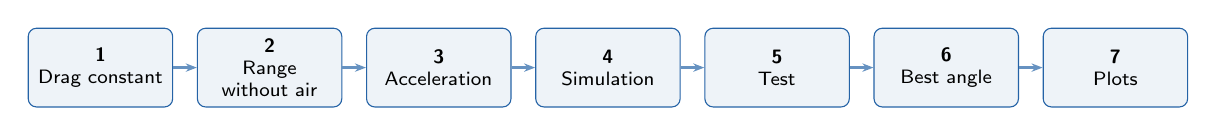
\begin{tikzpicture}[
  stage/.style={draw=task, fill=task!8, rounded corners=3pt, minimum height=1.0cm,
    text width=1.6cm, align=center, font=\sffamily\scriptsize},
  arr/.style={-{Stealth[length=4pt]}, thick, task!70},
  node distance=0.3cm]
  \node[stage] (a) {\textbf{1}\\Drag constant};
  \node[stage, right=of a] (b) {\textbf{2}\\Range without air};
  \node[stage, right=of b] (c) {\textbf{3}\\Acceleration};
  \node[stage, right=of c] (d) {\textbf{4}\\Simulation};
  \node[stage, right=of d] (e) {\textbf{5}\\Test};
  \node[stage, right=of e] (f) {\textbf{6}\\Best angle};
  \node[stage, right=of f] (g) {\textbf{7}\\Plots};
  \foreach \i/\j in {a/b, b/c, c/d, d/e, e/f, f/g} \draw[arr] (\i) -- (\j);
\end{tikzpicture}
\end{center}

% ---------------------------------------------------------------------------
\section{The Physics}
% ---------------------------------------------------------------------------
The ball starts on the ground and is kicked with speed $v_0$ at an angle $\theta$ above the horizontal. We use $x$ for the horizontal distance and $y$ for the height. The ball's starting velocity is
\begin{equation}
  v_x = v_0\cos\theta, \qquad v_y = v_0\sin\theta .
  \label{eq:initial}
\end{equation}

\begin{warning}
Python's \code{sin} and \code{cos} use \emph{radians}, but our angles are in degrees. Convert them first with \code{math.radians(angle\_deg)}.
\end{warning}

\subsection{Without air}
With only gravity acting, the ball follows a parabola and lands a distance
\begin{keyeq}[Key equation: range without air]
\vspace{-0.6em}
\begin{equation}
  R_\text{vac} = \frac{v_0^2 \sin 2\theta}{g}
  \label{eq:vac-range}
\end{equation}
\end{keyeq}
from where it started. This is largest when $\theta = \ang{45}$: the textbook answer that we want to test.

\subsection{With air}
The air pushes against the ball with a \emph{drag force}. This force always points opposite to the ball's motion, and it grows with the \emph{square} of the speed: a ball going twice as fast feels four times the drag.

\begin{center}
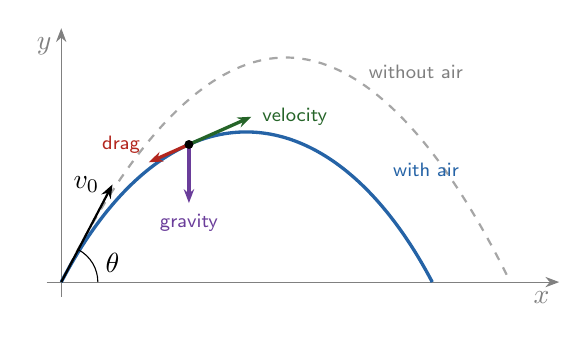
\begin{tikzpicture}[scale=0.62, >={Stealth[length=5pt]}]
  \draw[->, gray] (-0.3,0) -- (10.2,0) node[below left] {$x$};
  \draw[->, gray] (0,-0.3) -- (0,5.2) node[below left] {$y$};
  \draw[dashed, thick, gray!70] (0,0) parabola bend (4.6,4.6) (9.2,0);
  \node[gray, font=\sffamily\scriptsize, anchor=west] at (6.1,4.3) {without air};
  \draw[very thick, task] (0,0) .. controls (2.2,4.2) and (5.5,4.0) .. (7.6,0);
  \node[task, font=\sffamily\scriptsize, anchor=west] at (6.6,2.3) {with air};
  \draw[->, thick, black] (0,0) -- (1.05,2.0) node[left=1pt] {$v_0$};
  \draw (0.75,0) arc (0:62:0.75);
  \node at (1.05,0.4) {$\theta$};
  \coordinate (B) at (2.6156,2.8187);
  \draw[->, very thick, check!80!black] (B) -- ++(1.28,0.568) node[right, font=\sffamily\scriptsize] {velocity};
  \draw[->, very thick, warn] (B) -- ++(-0.82,-0.365) node[above left=-1pt, font=\sffamily\scriptsize] {drag};
  \draw[->, very thick, physics] (B) -- ++(0,-1.2) node[below, font=\sffamily\scriptsize] {gravity};
  \fill[black] (B) circle (2.6pt);
\end{tikzpicture}
\end{center}

Adding the drag force to gravity in Newton's second law gives the acceleration of the ball:

\begin{keyeq}[Key equations: acceleration with air resistance]
\vspace{-0.6em}
\begin{equation}
  a_x = -k\, v\, v_x, \qquad
  a_y = -g - k\, v\, v_y, \qquad
  \text{where}\quad v = \sqrt{v_x^2+v_y^2} \quad\text{and}\quad k = \frac{\rho\, C_d\, A}{2m}.
  \label{eq:accel}
\end{equation}
\end{keyeq}

Here $v$ is the speed of the ball, $\rho$ is the density of air, $C_d$ is the \emph{drag coefficient} (a number that describes how streamlined the ball is), $A = \pi r^2$ is the area of the ball's cross-section ($r$ is the radius, half the diameter) and $m$ is its mass. The \emph{drag constant} $k$ collects all of these into a single number, in units of \unit{\per\metre}. Setting $k = 0$ switches the air off. With drag there is no simple formula like \eqref{eq:vac-range} for the range, so we will find it with a simulation instead.

\textbf{Terminal velocity.} A ball dropped from a great height speeds up until the drag balances its weight. After that it falls at a steady \emph{terminal velocity}
\begin{equation}
  v_t = \sqrt{g/k} .
  \label{eq:terminal}
\end{equation}
This tells us how much drag matters. If the launch speed $v_0$ is much smaller than $v_t$, drag hardly matters; if $v_0$ is close to $v_t$ or larger, it matters a lot.

To keep things simple, we assume the ground is flat, there is no wind or spin, and $C_d$ does not change during the flight.

% ---------------------------------------------------------------------------
\section{The Simulation Method}
% ---------------------------------------------------------------------------
We follow the ball through its flight in small time steps of length $\Delta t$. If we know where the ball is and how fast it is moving \emph{now}, we can estimate where it will be a moment later, by assuming its velocity and acceleration hardly change during such a short step. This is called the \emph{Euler method}:

\begin{keyeq}[Key equations: one Euler step]
\vspace{-1.2em}
\begin{align}
  x_\text{new}   &= x   + v_x\,\Delta t, &
  v_{x,\text{new}} &= v_x + a_x\,\Delta t, \nonumber\\
  y_\text{new}   &= y   + v_y\,\Delta t, &
  v_{y,\text{new}} &= v_y + a_y\,\Delta t, \label{eq:euler}\\
  t_\text{new}   &= t + \Delta t, \nonumber
\end{align}
where $a_x$ and $a_y$ are calculated from \eqref{eq:accel} using the \emph{current} velocity $v_x$, $v_y$.
\end{keyeq}

We start at $x = y = 0$ with the velocity from \eqref{eq:initial} and repeat this step until the ball goes below the ground ($y < 0$). The $x$ position of that last point is the \emph{range} of the kick. A smaller $\Delta t$ gives a more accurate answer but needs more steps. Use $\Delta t = \qty{0.001}{\second}$ throughout.

% ---------------------------------------------------------------------------
\section{Tasks}
% ---------------------------------------------------------------------------
Work in a single Jupyter or Colab notebook, with a Markdown heading for each task. Use \emph{exactly} the function names and arguments given, because later tasks use the earlier functions. Give each function a short docstring. Each task ends with a \textcolor{check}{\sffamily\bfseries checkpoint}: make sure your numbers match before you move on.

% ===========================================================================
\task{Data and the drag constant}
Start your notebook with the imports and the data. Units are given in the comments.
\begin{pycode}
import math
import numpy as np
import matplotlib.pyplot as plt

G = 9.81      # gravitational acceleration (m/s^2)
RHO = 1.225   # density of air (kg/m^3)

# mass (kg), diameter (m), drag coefficient, launch speed (m/s)
football = {"mass": 0.430, "diameter": 0.220, "Cd": 0.25, "v0": 25.0}
\end{pycode}
Then write these two functions, using \eqref{eq:accel} and \eqref{eq:terminal}. Remember that the dictionary gives the \emph{diameter}, not the radius.
\begin{pycode}
def drag_constant(ball):
    """Return the drag constant k = RHO * Cd * A / (2 m), in 1/m."""

def terminal_velocity(k):
    """Return the terminal velocity sqrt(G / k), in m/s."""
\end{pycode}
Print $k$ and $v_t$ for the football.

\begin{checkpoint}
$k \approx \qty{0.01354}{\per\metre}$ and $v_t \approx \qty{26.92}{\metre\per\second}$. The football's launch speed, \qty{25}{\metre\per\second}, is close to $v_t$, so drag will matter a lot.
\end{checkpoint}

% ===========================================================================
\task{The range without air}
Write a function for the range without air, \eqref{eq:vac-range}. You will use it to test your simulation and to compare with the textbook answer.
\begin{pycode}
def vacuum_range(v0, angle_deg):
    """Return the range without air, in m."""
\end{pycode}

\begin{checkpoint}
\code{vacuum\_range(25, 45)} gives \qty{63.71}{\metre}. Angles of \ang{30} and \ang{60} both give \qty{55.17}{\metre}.
\end{checkpoint}

% ===========================================================================
\task{The acceleration}
Write a function for the acceleration with air resistance, \eqref{eq:accel}.
\begin{pycode}
def acceleration(vx, vy, k):
    """Return (ax, ay) for a ball with velocity (vx, vy) and drag constant k."""
\end{pycode}

\begin{checkpoint}
\code{acceleration(10, 0, 0)} gives \code{(0.0, -9.81)}: without drag, only gravity acts. With the football's $k$, \code{acceleration(20, 15, k)} gives about \code{(-6.7684, -14.8863)}.
\end{checkpoint}

% ===========================================================================
\task[task:simulate]{The simulation}
Write a function that uses the Euler method \eqref{eq:euler} to follow the ball until it hits the ground.
\begin{pycode}
def simulate_trajectory(v0, angle_deg, k, dt=0.001):
    """Simulate a kick until the ball goes below the ground.
    Return NumPy arrays t, x, y."""
\end{pycode}
Follow these steps:
\begin{enumerate}
  \item Set the starting values: $t = 0$, $x = 0$, $y = 0$, and $v_x$, $v_y$ from \eqref{eq:initial}.
  \item Create three lists, \code{ts}, \code{xs} and \code{ys}, each holding its starting value.
  \item \textbf{While} $y \ge 0$:
  \begin{enumerate}[label=(\alph*)]
    \item calculate \code{ax, ay} by calling \code{acceleration(vx, vy, k)};
    \item update \code{x}, \code{y}, \code{vx}, \code{vy} and \code{t} using \eqref{eq:euler};
    \item append the new \code{t}, \code{x} and \code{y} to the three lists.
  \end{enumerate}
  \item Convert the three lists to NumPy arrays and return them.
\end{enumerate}
The last point in the arrays is the first one below the ground, so the range is \code{x[-1]}.

\begin{warning}
Update \code{x} and \code{y} \emph{before} you change \code{vx} and \code{vy}. The position update must use the velocity from the start of the step. If your loop never ends, the ball is not coming down: check the sign of $g$ in your acceleration.
\end{warning}

\begin{checkpoint}
For the football at \ang{45}, the arrays have 3127 elements and the flight lasts about \qty{3.13}{\second}. The highest point (\code{y.max()}) is about \qty{12.06}{\metre} and the range is about \qty{39.61}{\metre}: almost 40\% shorter than the \qty{63.71}{\metre} without air!
\end{checkpoint}

% ===========================================================================
\task[task:verify]{Testing the simulation}
Before trusting a simulation, we should test it on a case where we already know the answer. With $k = 0$, your simulation should give the same range as \code{vacuum\_range}. For $v_0 = \qty{25}{\metre\per\second}$ and \ang{45}, print the simulated range, the exact range, and the relative error
\begin{equation*}
  \varepsilon = \frac{\left|R_\text{sim} - R_\text{exact}\right|}{R_\text{exact}} .
\end{equation*}

\begin{checkpoint}
\qty{63.746}{\metre} against \qty{63.710}{\metre}, so $\varepsilon \approx 5.5\times10^{-4}$. If your error is much bigger than $10^{-3}$, there is a bug in your simulation: check the warning in Task~\ref{task:simulate}.
\end{checkpoint}

% ===========================================================================
\task[task:brute]{Finding the best angle}
There is no formula for the best angle with air resistance, so we simply try every whole-degree angle from \ang{1} to \ang{89} and see which one goes furthest.
\begin{pycode}
def range_vs_angle(v0, k, dt=0.001):
    """Return NumPy arrays of angles (1 to 89 degrees) and their ranges."""
\end{pycode}
Loop over \code{range(1, 90)}. For each angle, run \code{simulate\_trajectory} and append the angle and its range (\code{x[-1]}) to two lists. Return them as NumPy arrays.

Then, for the football, find and print the best angle and its range. Also print the textbook range (no air, \ang{45}) and the ratio of the two ranges.

\begin{hint}
\code{i = np.argmax(ranges)} gives the \emph{position} of the largest range in the array. The best angle is then \code{angles[i]}.
\end{hint}

\begin{checkpoint}
The best angle is \ang{41}, with a range of \qty{39.87}{\metre}, compared with \qty{63.71}{\metre} without air: a ratio of $0.626$.
\end{checkpoint}

% ===========================================================================
\task{Plots}
Make the following two figures. Each needs axis labels with units, a title, and a legend.
\begin{enumerate}
  \item \textbf{Trajectories.} Plot $y$ against $x$ for the football kicked at \ang{15}, \ang{30}, \ang{45}, \ang{60} and \ang{75}. Show each angle with air (solid line) and without air (dashed line, same colour, using $k = 0$). Use \code{ax.set\_aspect("equal")} so the shapes are not squashed.
  \item \textbf{Range against angle.} Plot the ranges from Task~\ref{task:brute} against the angle. On the same axes, plot \code{vacuum\_range} for the same angles. Mark the highest point of each curve.
\end{enumerate}

\begin{hint}
To give a solid and a dashed line the same colour, pass \code{color=f"C\{i\}"} to both \code{plot} calls, where \code{i} counts 0, 1, 2, \dots{} through the angles.
\end{hint}

% ---------------------------------------------------------------------------
\section{Written Questions}
% ---------------------------------------------------------------------------
Answer these in Markdown cells at the end of your notebook, in a few sentences each, using your own results and plots.
\begin{enumerate}
  \item Why is the best angle with air resistance less than \ang{45}? \emph{(Think about how long the ball stays in the air at steep angles, and how drag depends on speed.)}
  \item In your trajectory plot, the balls with air resistance come down more steeply than they go up. Why?
  \item Why is it useful to test the simulation with $k = 0$? What happens to the error in Task~\ref{task:verify} if you make $\Delta t$ ten times smaller? Try it.
  \item The football's launch speed is close to its terminal velocity. Use this to explain why drag shortens its range so much. Would drag matter more or less for a gentle kick at \qty{10}{\metre\per\second}? Check with your code.
\end{enumerate}

% ---------------------------------------------------------------------------
\section{Submission and Marking}
% ---------------------------------------------------------------------------
Submit your notebook (\code{.ipynb}) on the VLE. Before you submit, choose \emph{Restart and run all} (in Colab: \emph{Runtime} $\to$ \emph{Restart and run all}) and check that it runs from top to bottom without errors. In Colab, download it with \emph{File} $\to$ \emph{Download} $\to$ \emph{Download .ipynb}.

\begin{center}
\small
\begin{tabular}{@{}lr@{\qquad\qquad}lr@{}}
  \toprule
  \textbf{Component} & \textbf{Weight} & \textbf{Component} & \textbf{Weight} \\
  \midrule
  Task 1: Drag constant      & 5\%  & Task 6: Best angle                     & 15\% \\
  Task 2: Range without air & 5\%  & Task 7: Plots                          & 15\% \\
  Tasks 3--4: Simulation     & 30\% & Code clarity (layout, docstrings, comments) & 10\% \\
  Task 5: Testing            & 5\%  & Written questions                      & 15\% \\
  \bottomrule
\end{tabular}
\end{center}

\end{document}
